
\section{Обзор литературы}
\subsection{Базовые определения}
Рассотротрим вероятностное просранство $(X, \Theta, p)$, где $X$ просранство, $\Theta$ сигма- алгебра на $X$, $p$ вероятносная мера введеная на сигма-алгебре $\Theta$.
Тогда введем энтропию
\begin{gather}
\begin{aligned}  
H[X] = - \EX_{p(x)}\log(p(x))
\end{aligned}
\end{gather}
В дискретном случае
\begin{gather}
\begin{aligned}  
H[X] = - \sum_{x \in X}p(x)\log(p(x))
\end{aligned}
\end{gather}
Введем совместную энтропию
\begin{gather}
\begin{aligned}  
H[X, Y] = - \EX_{p(x, y)}\log(p(x, y))
\end{aligned}
\end{gather}
В дискретном случае
\begin{gather}
\begin{aligned}  
H[X, Y] = - \sum_{x \in X, y \in Y}p(x, y)\log(p(x, y))
\end{aligned}
\end{gather}
Теперь введем условную энтропию
\begin{gather}
\begin{aligned}  
    H[X | Y] = - \EX_{p(x, y)}\log(p(x | y)) = H[X, Y] - X[Y] \\
\end{aligned}
\end{gather}
\begin{gather}
\begin{aligned}
    \Box \: H[X, Y] - X[Y] = - \EX_{p(x, y)}\log(p(x, y)) + \EX_{p(y)}\log(p(y)) =  \\
    - \int_{x, y}p(x, y)\log(p(x, y)) + \int_{y}p(y)\log(p(y)) = \\
    - \int_{x, y}p(x, y)\log(p(x, y)) + \int_{y}\sum_{x}p(y, x)\log(p(y)) = \\ 
    - \int_{x, y}p(x, y)\log(p(x, y)) + \int_{x, y}p(y, x)\log(p(y)) = \\ 
    - \int_{x, y}p(x, y)(\log(p(x, y)) - \log(p(y))) = \\ 
    - \int_{x, y}p(x, y)(\log(p(x, y) / p(y))) = - \int_{x, y}p(x, y)\log(p(x | y)) = H[X | Y] \:\Box
\end{aligned}
\end{gather}    
Теперь введем информацию между двумя величинами
\begin{gather}
\begin{aligned}
    I[X, Y] = - \EX_{p(x, y)}\log(\frac{p(x)p(y)}{p(x, y)}) = H[X] + H[Y] - H[X, Y]
\end{aligned}
\end{gather}    
\begin{gather}
\begin{aligned}
    \Box \: H[X] + H[Y] - H[X, Y] = \\ 
    - (\int_{x, y}p(y, x)\log(p(x)) + \int_{x, y}p(x, y)\log(p(y)) - \int_{x, y}p(y, x)\log(p(x, y))) = \\
    - \int_{x, y}p(y, x) (\log(p(x)) + \log(p(y)) - log(p(x, y))) = \\
    - \int_{x, y}p(x, y)\log(\frac{p(x)p(y)}{p(x, y)}) = I[X, Y] \:\Box 
\end{aligned}
\end{gather}    
\subsection{Информационные множества}
Таким образом информационные эвристики можно воспринимать как множественные операции
\begin{center}
    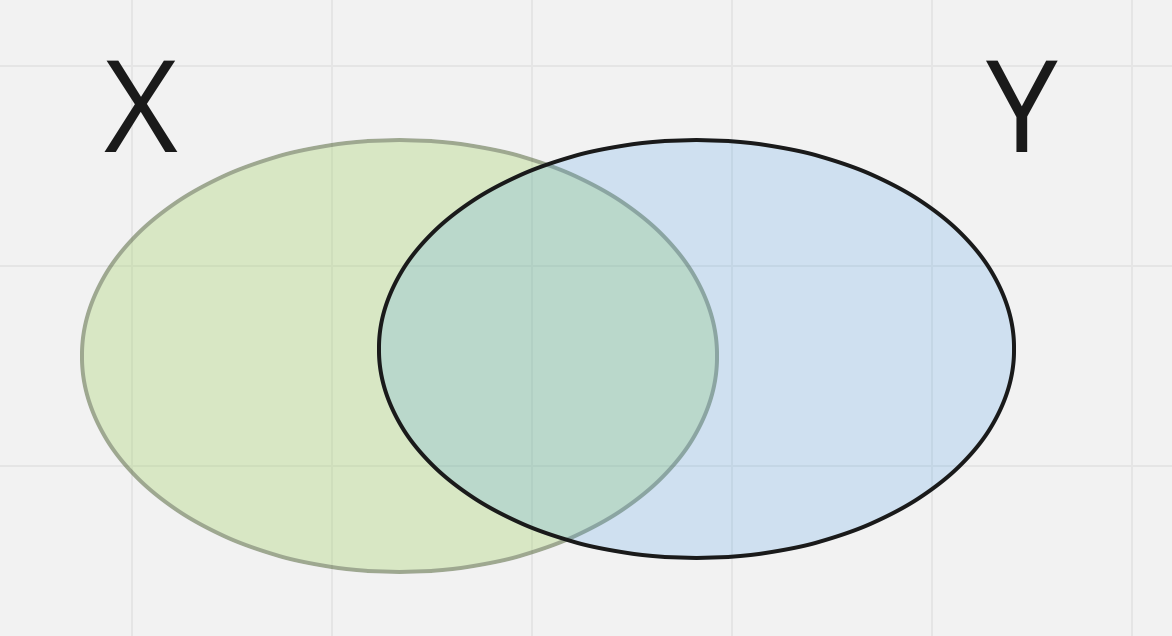
\includegraphics[scale=0.4]{images/information_sets.png}
\end{center}
Рассмотрим пространства $X$ и $Y$ как множества, тогда мощностью множества
\begin{enumerate}
\item $|X|$ будем называть $H[X]$
\item $|Y|$ будем называть $H[Y]$
\item $|X \cap Y|$ будет $I[X, Y]$
\item $|X \cup Y|$ будет $H[X, Y]$
\item $|X \setminus Y|$ будет $H[X | Y]$
\item $|Y \setminus X|$ будет $H[Y | X]$
\end{enumerate}
Перейдем к рассмотрению информационных множеств в рамках нейронных сетей. Тогда $X$ рассмотрим как пространство входных данных, $Y$ рассмотрим как пространство выходных данных, $Z$ как латентное пространство. Визуализируем их в качестве множеств. Подобная диаграмма называется Mickey Mouse I-diagram.
\begin{center}
    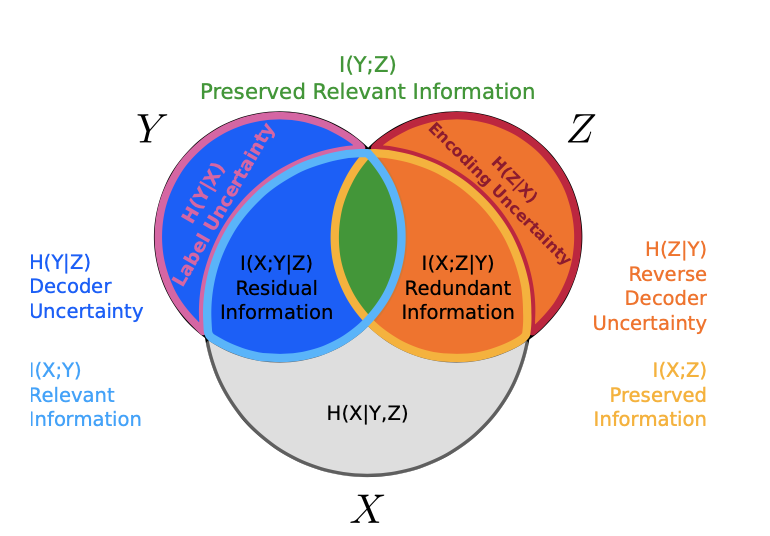
\includegraphics[scale=1.]{images/micky_mouse_diagram.png}
\end{center}
Соответственно каждое из подмножеств численно вычисляется с помощью информационных метрик. Заметим, что $X \cap Y \cap Z = Y \cap Z$, иными словами $I[X, Y, Z] = I[Y, Z]$. Докажем это. $I[X, Y, Z] = I[Y, Z] \Leftrightarrow I[Y, Z] - I[X, Y, Z] = H[Y, Z | X] = 0$. Это верно, так как для каждого входа $x_i \in X$ зафиксирован конкретный выход $y_i \in Y$ и конкретное латентное кодирование $z_i \in Z$, а значит пространство $(Y, Z | X)$ будет одномерно для каждого $x_i \in X$, следовательно $H[Y, Z | X] = 0$.
\subsection{Information Bottleneck Principe}
Задача нейронной сети вычленить всю релевантую информацию из входа $X$ описывающую выход $Y$. Оптимальное отображение будет отбрасывать всю нерелевантную информацию, таким образом задача обучения состоит в том, чтобы минимизировать общую информацию $I[X, Z]$, при этом сохраняя всю необходимую общую информацию между выходом и латентным пространством $I[Y, Z]$. Обощая эти факты, поиск оптимального решения описывается задачей оптимизации (IB):
\begin{gather}
\begin{aligned}
min_{Z} I[X, Z] - \beta * I[Z, Y]
\end{aligned}
\end{gather}
Где $\beta$ оператор компромиса между информацией репрезентации $I[X, Z]$, и информацией релевантной информации $I[Z, Y]$. Посмотрев на Mickey Mouse I-diagram можно заметить, что множество $Z$ пытается максимально влится в $Y$ и иметь наименьшее пересечение с $X$. Проверим данные гипотезы на практике.








